\documentclass[11pt]{beamer}
\usetheme{Malmoe}
\usepackage[utf8]{inputenc}
\usepackage{amsmath}
\usepackage{amsfonts}
\usepackage{amssymb}
\usepackage{graphicx}
\graphicspath{{./src/}}
%\author{}
%\title{}
%\setbeamercovered{transparent} 
%\setbeamertemplate{navigation symbols}{} 
%\logo{} 
%\institute{} 
%\date{} 
%\subject{} 
\title{Nanospace Link Budget Calculation UI}
\subtitle{}
\author{Julien Prissimitzis}
\date{\today}

\setbeamercolor{block title}{use=structure,fg=white,bg=blue!60!black}
\setbeamercolor{block body}{use=structure,fg=black,bg=blue!10!white}
\setbeamertemplate{blocks}[rounded][shadow=false]

\begin{document}

%\begin{frame}
%\titlepage
%\end{frame}

%\begin{frame}
%\tableofcontents
%\end{frame}
\begin{frame}
	\titlepage
\end{frame}

\section{Link Budget \& Context}

\begin{frame}
	\frametitle{Link Budget \& Context}
%\textbf{Goal:} Communication with a satellite

%\textbf{Link budget? }%\textit{An accounting of all of the power gains and losses that a communication signal experiences (Wikipedia)} 

	\begin{block}{Link Budget ?}
	  $P_{received}(dB) = P_{transmitted}(dB) + G_{dB} - L_{dB}$
	\end{block}


%Multiple sources of 
	Losses : FSL, antenna depointing, polarization, edge of coverage, technological, rain attenuation, ... %$\Rightarrow$  Tool keeping track of everything
	\pause
%\textbf{Current Tools:}
%\begin{block}{Some tools:}
	\begin{columns}[onlytextwidth]
		\begin{column}{.32\textwidth}
			\begin{figure}
				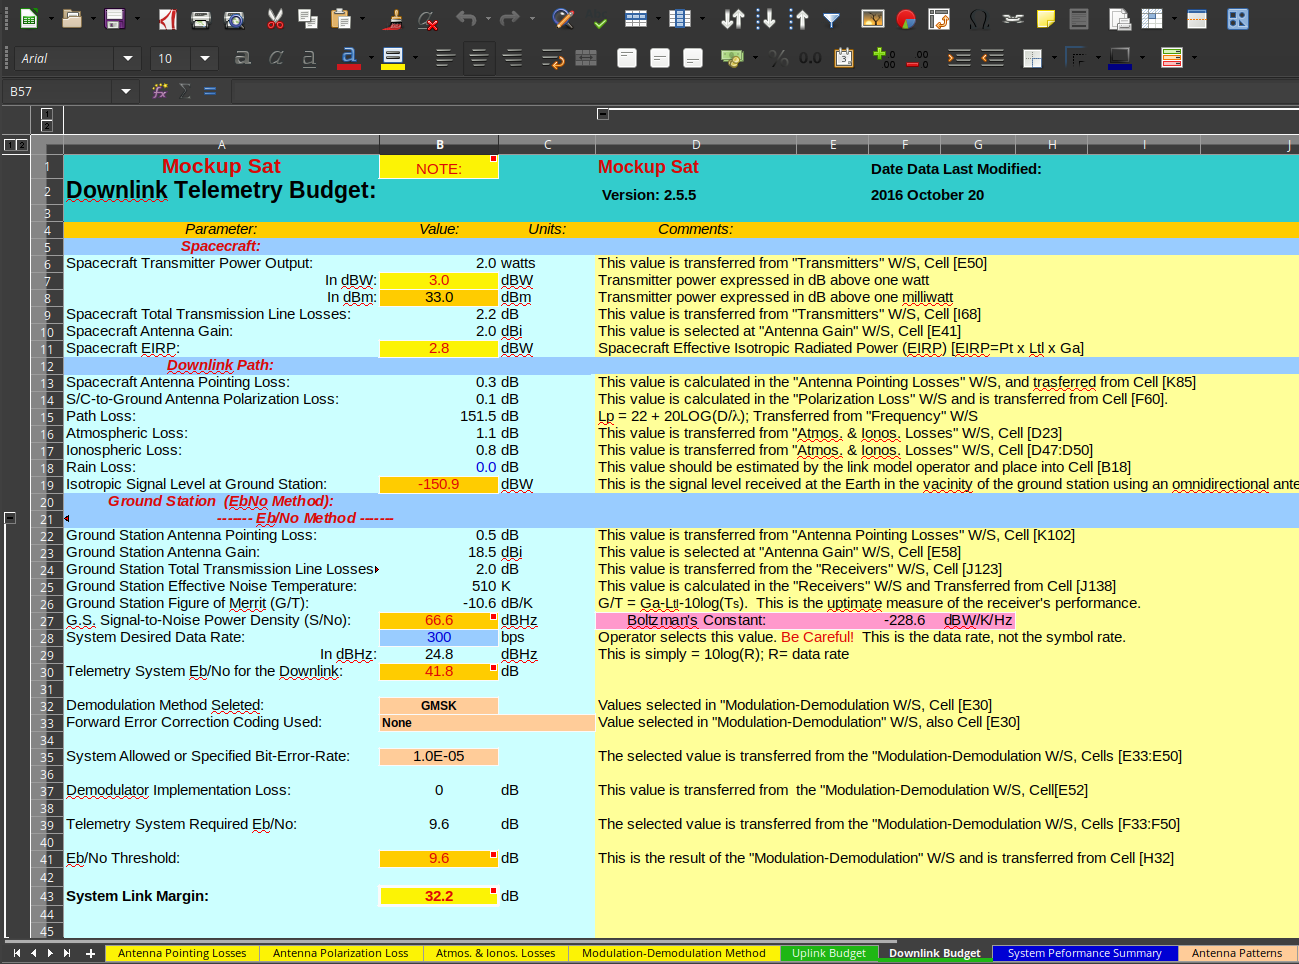
\includegraphics[width=\textwidth]{AMSAT.png}
				\caption{AMSAT.xls}
			\end{figure}
		\end{column}
		\hfill
		\begin{column}{.32\textwidth}
			\begin{figure}
				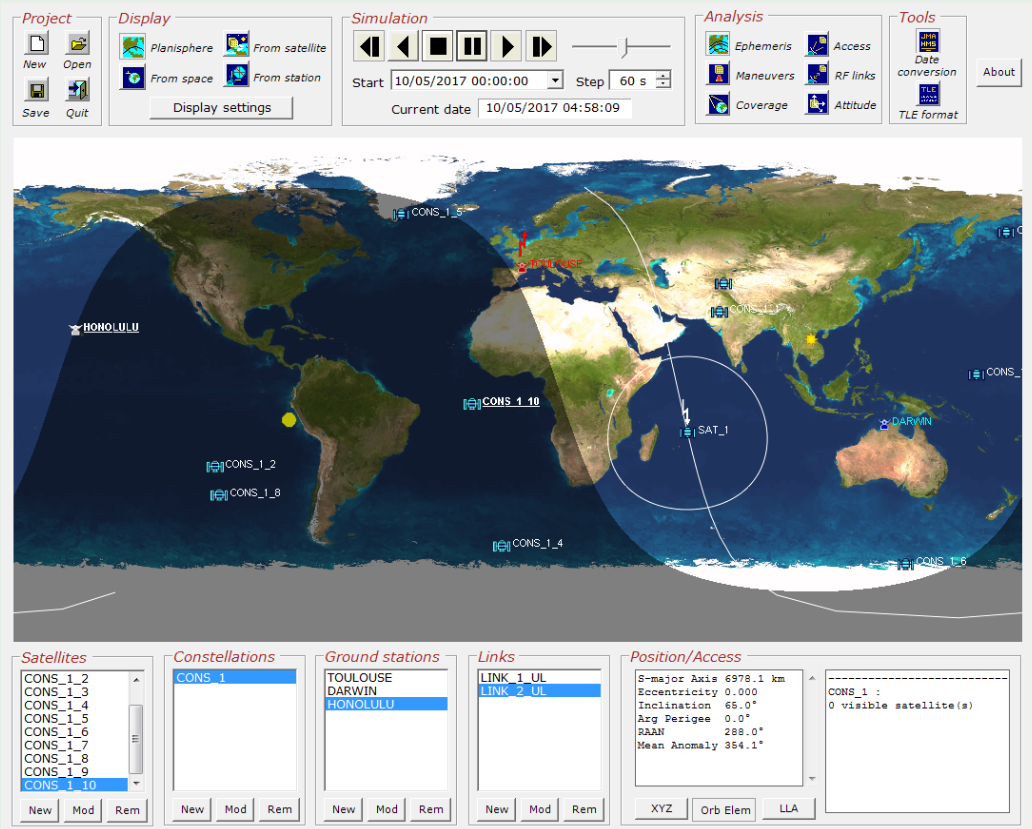
\includegraphics[width=\textwidth]{satorb.png}
				\caption{SatOrb}
			\end{figure}
		\end{column}
		\hfill
		\begin{column}{.28\textwidth}
			Python libraries : 
			\begin{itemize}
				\item linkpredict
				\item luplink
				\item ...
			\end{itemize}
		\end{column}
	\end{columns}
\end{frame}

\section{Project}

\begin{frame}
	\frametitle{Project}
	Open-source tool interfacing with NSS (inside JSatOrb)
	\begin{columns}[onlytextwidth]
		\begin{column}{.55\textwidth}
		\begin{figure}
			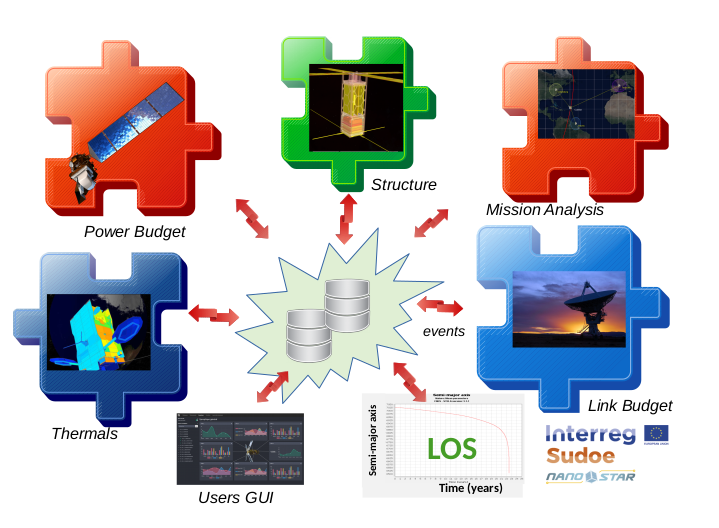
\includegraphics[width=.8\textwidth]{nss.png}
			\caption{Nanospace Software Suite (NSS)}
		\end{figure}
	\end{column}
	\hfill
	\begin{column}{.5\textwidth}
	Requirements : 
	\begin{itemize}
		\item Usable inside NSS
		\item Suitable for teaching
		\item Modular \& easily extendable
		\item Unit-tested
	\end{itemize}
	\end{column}
\end{columns}
%With web application frameworks, easy to build modular apps
\end{frame}

\begin{frame}
	\begin{figure}
		\frametitle{Current advancement}
		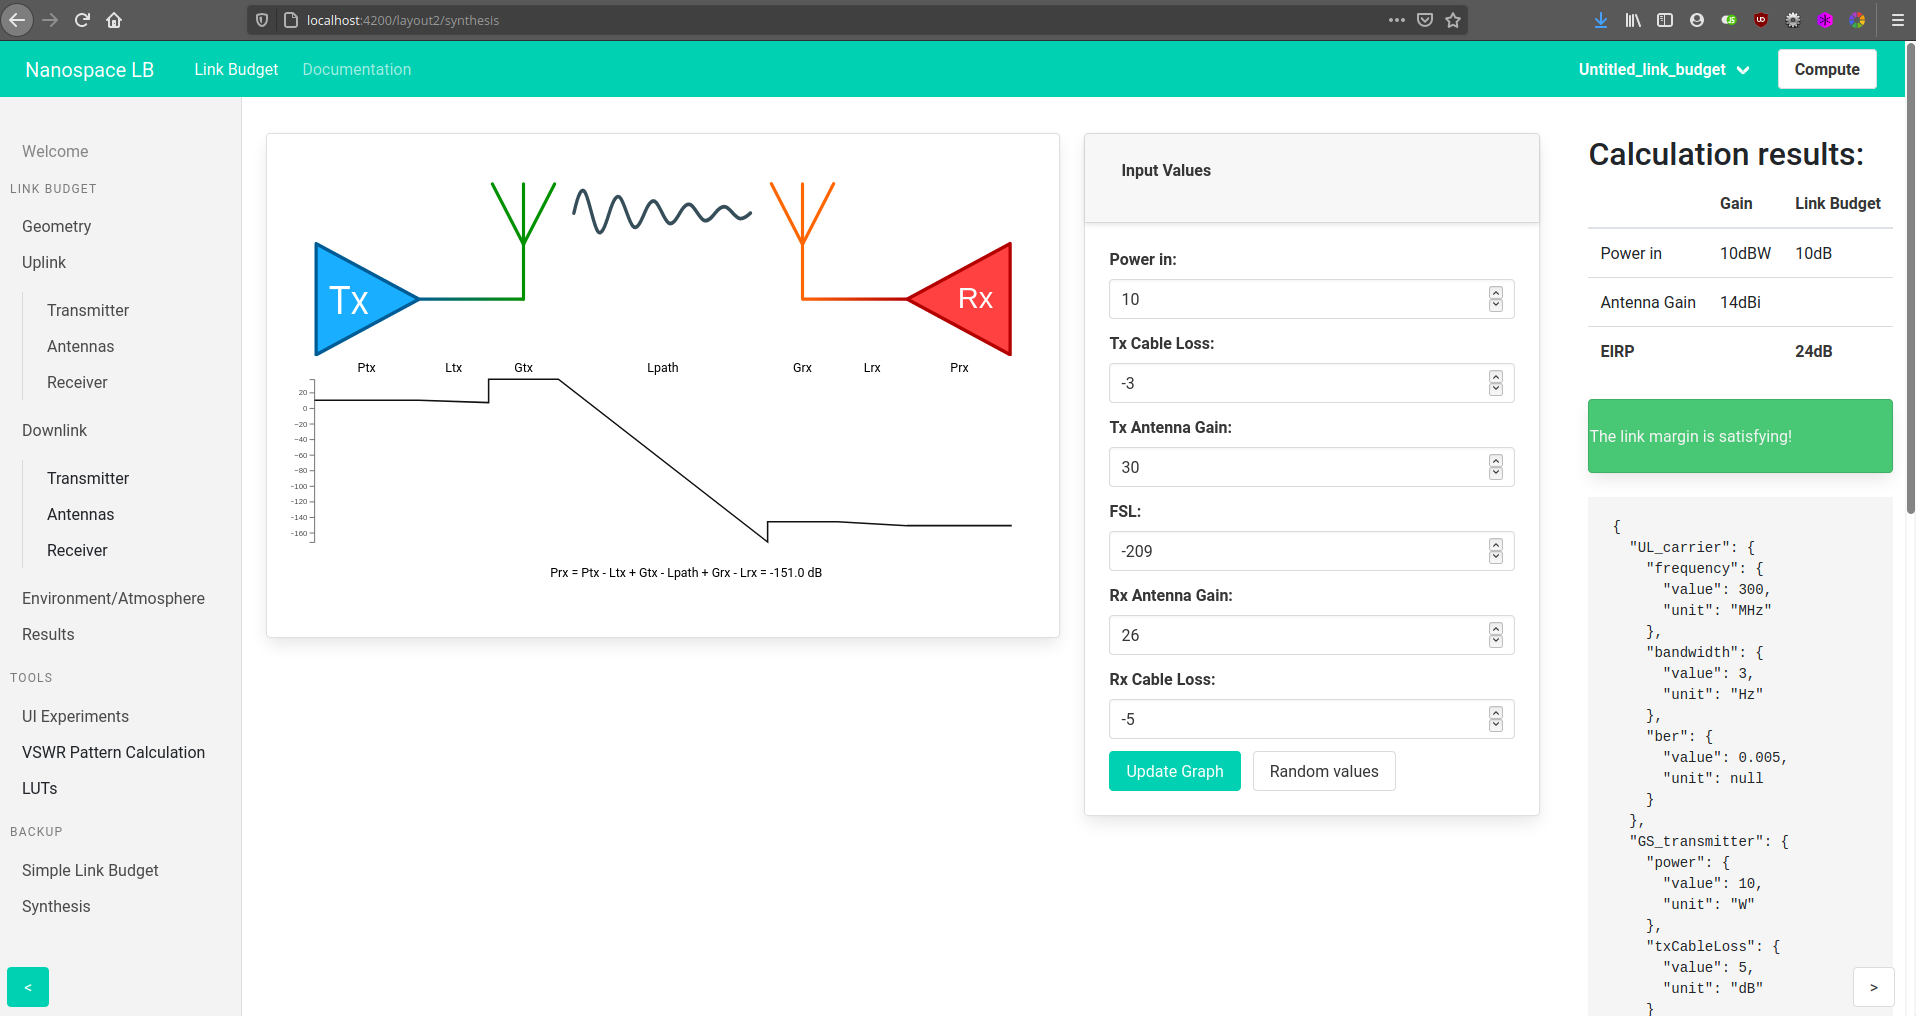
\includegraphics[width=\textwidth]{nlb.png}
			\caption{What it currently looks like}
	\end{figure}
\end{frame}

\begin{frame}
\begin{columns}[onlytextwidth]
	\begin{column}{0.4\textwidth}
		\begin{figure}
			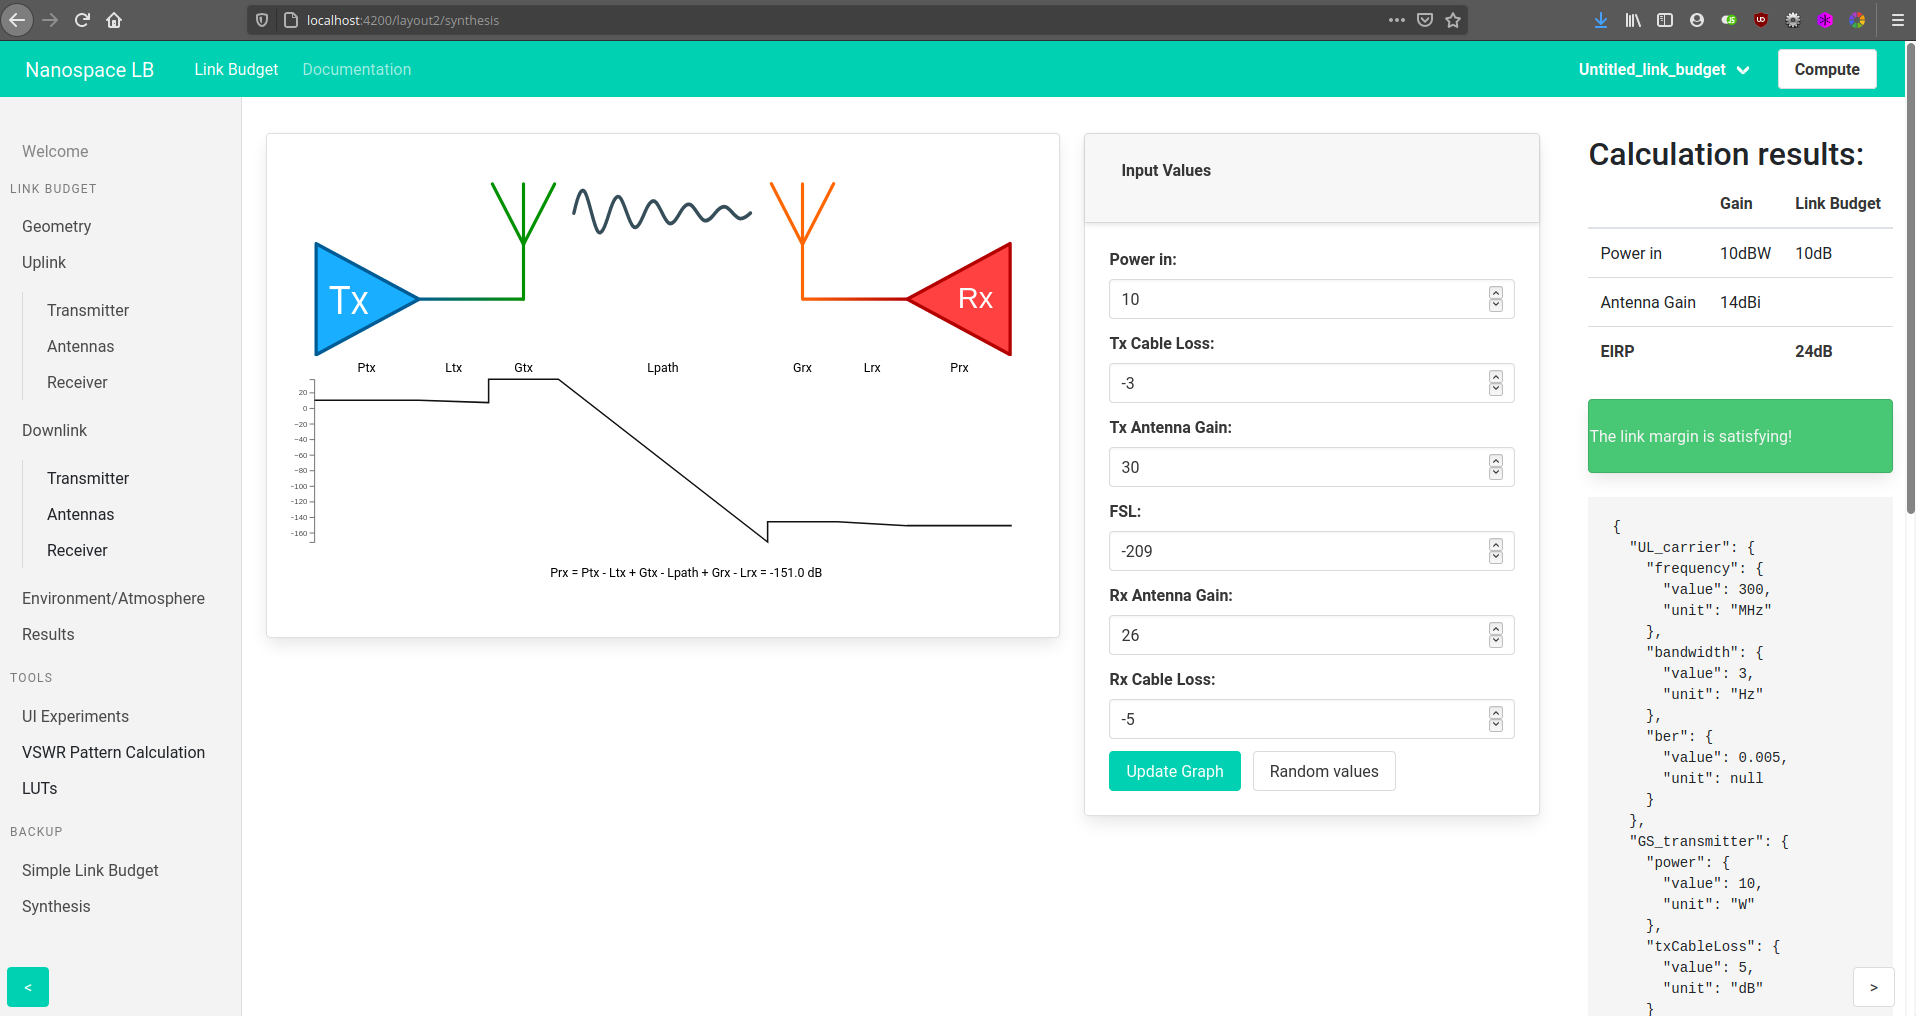
\includegraphics[width=\textwidth]{nlb.png}
			\caption{Current UI}
		\end{figure}
	\end{column}
	\hfill
	\begin{column}{0.45\textwidth}
		\textbf{Angular framework :} 
		\begin{itemize}
			\item Components,
			\item Typescript,  
			\item Good testing capabilities
		\end{itemize}
		\bigbreak
	\end{column}
\end{columns}
\end{frame}

\begin{frame}
	\frametitle{Some challenges}
	\begin{columns}[onlytextwidth]
		\begin{column}{0.45\textwidth}
			\begin{itemize}
				\item Lots of inputs
				\item Fit most use cases
			\end{itemize}
		\end{column}
		
		\begin{column}{0.6\textwidth}
			\begin{figure}
				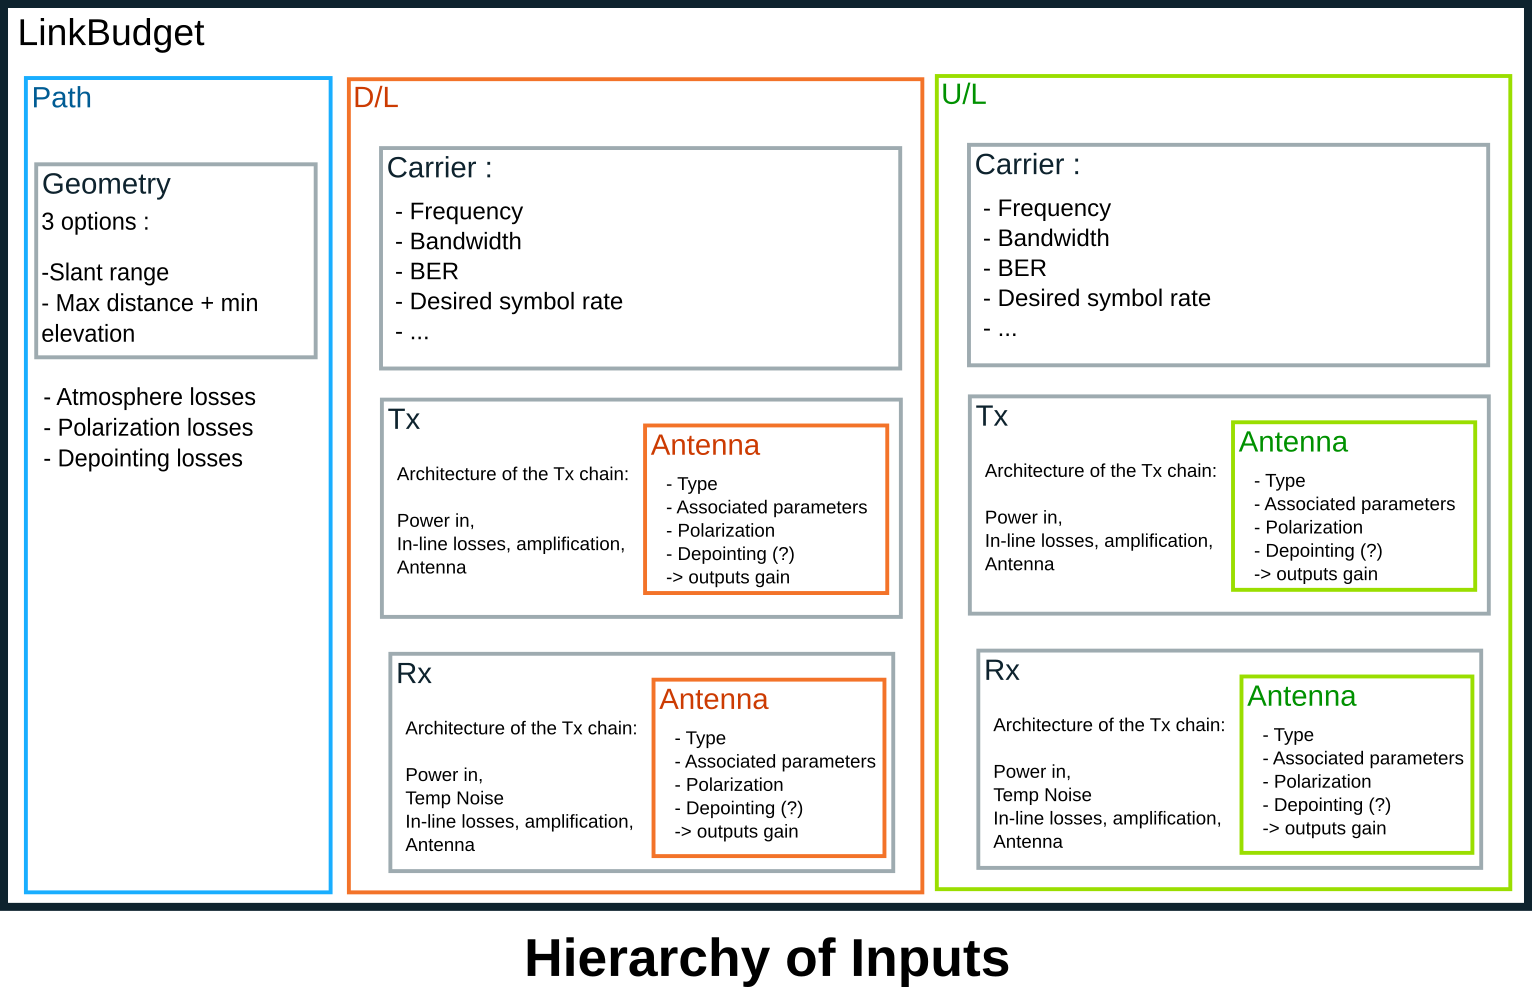
\includegraphics[width=\textwidth]{hierarchSimplified.png}
				%\caption{Current UI}
			\end{figure}
		\end{column}
		
		\hfill
	\end{columns}
\end{frame}

\begin{frame}
\frametitle{Currently}
	\begin{columns}[onlytextwidth]
		\begin{column}{0.5\textwidth}
			\begin{itemize}
				\item Form Logic
				\item D3.js graph
				\item Angular \& CSS capabilities
			\end{itemize}
			\begin{figure}[hbtp]
			\centering
				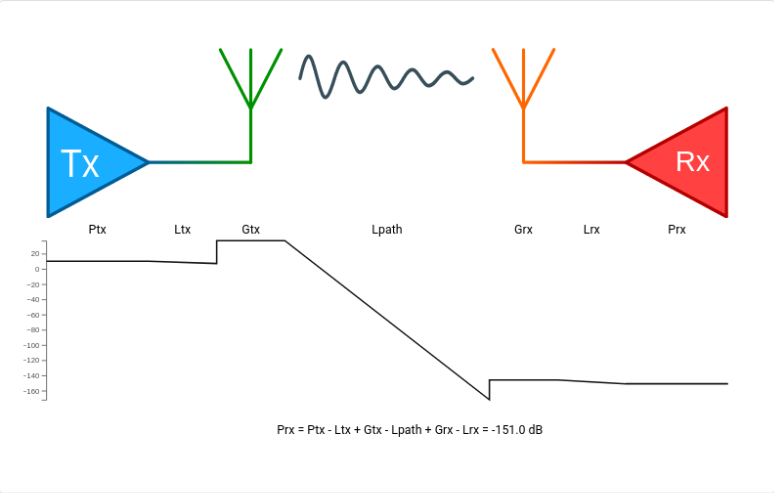
\includegraphics[width=\textwidth]{src/d3.png}
				\caption{Form Architecture}
			\end{figure}
%			Next steps : 
%			\begin{itemize}
%			\item Full static link budget 
%			\item Dynamic link budget
		%Next :
		%\end{itemize}
		\end{column}
		\hfill
		\begin{column}{0.4\textwidth}
			\begin{figure}[hbtp]
				\centering
				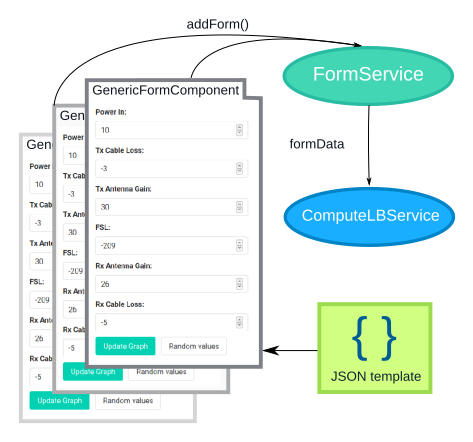
\includegraphics[width=\textwidth]{src/formArchSimplified.png}
				\caption{Form Architecture}
			\end{figure}
			
		\end{column}
	\end{columns}
	%UX issues : enough clarity while providing easy way to input data
	%\textit{Difficulties : juggling with many options}
	
\end{frame}

\end{document}


